\documentclass[times, 10pt,twocolumn]{article}
\usepackage{mapnoreduce-report-g03}
\usepackage{times}
\usepackage{graphicx}
\usepackage[utf8x]{inputenc}
\usepackage{enumitem}
\usepackage{mathtools}
\usepackage{bm}
\usepackage{breqn}
\usepackage{wasysym}
\usepackage{amsfonts}
\usepackage{amssymb}
\usepackage{graphicx}
\usepackage{fixltx2e}
\usepackage{color}
\usepackage{colortbl}
\usepackage{subfig}
\usepackage{url}
\usepackage{cite}
\usepackage[portuguese, english]{babel}
\usepackage{threeparttable}
\PassOptionsToPackage{hyphens}{url}\usepackage{hyperref}
\usepackage[hyphens]{url}
\hypersetup{breaklinks=true}
\usepackage[square,sort,comma,numbers]{natbib}
\usepackage{tabularx}
\usepackage{booktabs}
\usepackage{chngpage}
\usepackage{pdflscape}
\usepackage[table]{xcolor}
\definecolor{lightgray}{gray}{0.9}
\usepackage{tikz}
\usepackage[printonlyused,nolist]{acronym}

\makeatletter
\g@addto@macro{\UrlBreaks}{\UrlOrds}
\makeatother

\pagestyle{empty}

\begin{document}
	\title{MapNoReduce Platform}

	\author{
        João Pinho\\jpe.pinho@gmail.com
        \and Diogo Rosa\\diogo.m.c.rosa@gmail.com
        \and Cláudia Filipe\\claudiapbfilipe@gmail.com\\\\
		\and Instituto Superior Técnico\\
        Middleware for Distributed Internet Applications\\
        Lisbon, Portugal
    }
	\maketitle
	\thispagestyle{empty}

    % region: acronyms %
    \acrodef{MNRP}{MapNoReduce Platform}

	\begin{abstract}
		This project consists in the design and implementation of \ac{MNRP}, a simplified implementation of the MapReduce middleware and programming model. This platform extracts the input key/value pairs from input files and distributes the Map calls, called Jobs, across multiple machines, the Workers.
		Also, the platform ensures a good performance by monitoring job's progress, detecting faulty or slow machines and rescheduling their tasks on idle machines. That is assured by Job Trackers, which are distributed in this platform, in contrast to the original implementation of MapReduce, where they are centralized. This mechanism was implemented inspired in Facebook's solution—Corona~\cite{Facebook2012}.
		Additionally, in order to test the platform it was developed a PuppetMaster component which allows to control the platform, and also to induce some delays and faults to the system in order to perform some tests and evaluation.
	\end{abstract}

	\section{Introduction}
	MapReduce was introduced by Google in 2004~\cite{Dean2008} and is currently one of the most popular approaches for large scale data analytics - also thanks to the availability of high quality open-source implementations. When using the MapReduce paradigm, the computation takes a set of input key/value pairs, and produces a set of output key/value pairs. MapReduce users express the computation as two functions: Map and Reduce.
	This project focuses only the Map part, which uses a Map function given by the user and an input set of key/value pairs to produce a set of key/value pairs.
	In \ac{MNRP} the keys are the numbers of the line of the file being read and the values are the content of those lines.
    The Map invocations, called Jobs, are distributed across multiple machines by automatically partitioning the input data into a set of splits of size S. The input splits can be processed in parallel by those machines, named Workers. The system ensures that for each job submitted, all the input data is processed with a good performance through the monitoring of jobs' progress, fault or slow machines detection and reschedule of idle machine's tasks.
	In the original MapReduce implementation these tasks are performed by the JobTracker which is a centralized component. If the JobTracker fails the system can't receive new jobs nor processing pending ones, which can be critical in systems that need high availability.
	Considering JobTracker as a single point of failure~\cite{Kalavri2013}, it is necessary to replicate this component. As it would add complexity to the system and overhead, this project also introduces a new entity, the CoordinationManager, separating cluster resource management from job coordination, which allows the system to focus on make faster scheduling tasks.

	\section{MapNoReduce Architecture}

        \ac{MNRP} is a simplified implementation of the MapReduce middleware and programming model, focused on the Map part. On this simplified version, our work provides a solution to common problems related with the reference architecture of the MapReduce platform. Those problems are related with fault-tolerance, replication and performance and will be discussed in the next sections. Additionally, we added some features that enable the overall testing of the system, such as the ability to run scripts over one or more functional servers or the capacity to monitor the system state while running those scripts.

        \begin{figure}[!h]
            \begin{center}
                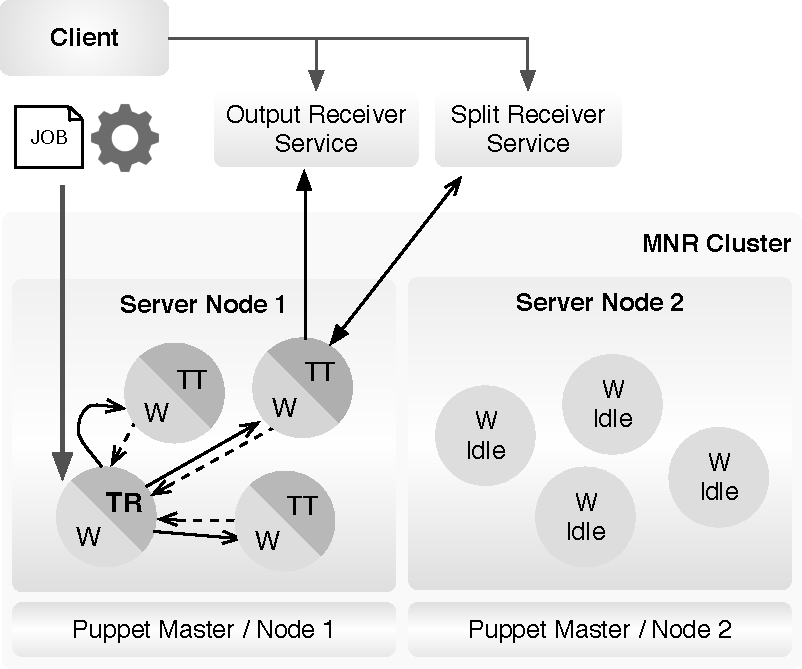
\includegraphics[width=0.48\textwidth]{pics/architecture.pdf}
                \caption{We illustrate an example of the MapNoReduce architecture. We represent one cluster with two server nodes. Inside the processing node, one JobTracker coordinates with other TaskTrackers to process the client job.  }
                \label{fig:mnr-architecture}
            \end{center}
        \end{figure}

    	\subsection{Worker}

        In \ac{MNRP}, workers are simple .NET Remoting Services that receive requests on a given endpoint, known as \emph{Service URI}.

        Every time a job gets submitted to the \ac{MNRP}, an entry worker gets selected to handle its processing. Workers are therefore, available working units that in a given \emph{Server Node} represent its work capacity. This is, for a given server node with 10 workers, such node has capacity to parallelize work to 10 workers.

        The \emph{Service URI} of a worker is composed by 4 parts, starting with the protocol, followed by the \emph{host name}, the \emph{host port}, and finally the worker identifier. An example of such a \emph{Service URI} would be something like \emph{{\small tcp://192.168.1.74:20001/W1}}, representing the endpoint for the worker 1 in the server node.
        
        It is also worth mentioning that, since a worker is no more than a thread waiting for requests on a given server node—represented by a physical machine,—workers share the same machine resources among them when running in parallel, if all located in the same server node obviously.

        When a worker gets selected by a client application as entry worker, it is made responsible for the correct processing of that job. This means that it must keep track of all the splits that must be processed for that job, what is their status, whose worker is processing each split and in case of a failure it must reassign the lost split to another worker, re-executing the job split if necessary.

        On the other end, each worker that receives the job of processing a given job's split, must report progress to the entry worker in regular intervals, to let it know that the job split is being processed without any problems.

        In the \ac{MNRP}, to an entry worker responsible of managing the processing of a whole job we call, Task Runner and to a worker that reports progress to the Task Runner we call Task Tracker.
        
        Note that, on a real world setup, ideally workers would be distributed by various machines within a cluster. In our work we opted to segment those workers differently within threads, were each machine running our solution acts like a cluster with multiples workers. This decision enabled us to test the system with few resources, since we do not have a cluster of machines at our disposal.

    	\subsection{Job Tracker}

        The overall execution and progress tracking of a job is handled by Job Trackers. In \ac{MNRP} \emph{Job Trackers} can have two distinct roles: they could be responsible for the distribution of splits for a given job, or they could be responsible for reporting progress about the processing of a given split.

            \subsubsection{Task Runner}

            When an entry worker receives a job, it is forced to split between two functions: {\it (i)} keep listening for requests for processing new jobs, and {\it (ii)} keep track of the job just received. To achieve the point in {\it (ii)}, the worker creates a \emph{Task Runner} on a new thread, enabling it to keep processing requests without getting blocked while the Task Runner is active.

            Conversely, while the \emph{Task Runner} is actively managing a job, there is no guarantee that no other job arrives during its execution. To avoid blocking incoming requests, we use a FIFO queue, to postpone the execution of jobs received while a job is being handled.

            A \emph{Task Runner} is continuously polling the jobs queue, to check whether it should terminate or process a new job from the queue. In our solution, we decided to terminate the \emph{Task Runner} when there are no jobs, to avoid having a thread wasting resources without any purpose. Because of this, whenever a worker receives a new job it must first determine if it needs to invoke a new \emph{Task Runner} to process the job.

            Finally, the processing of a job can take some time to complete, because of this, the \emph{Task Runner} delegates such processing to a dedicated thread and blocks itself waiting for it to terminate. Note that, the worker thread runs in separate of the \emph{Task Runner}, therefore while the \emph{Task Runner} is blocked its jobs queue can still be updated by the entry worker. The dedicated thread that processes a give job, also known as Job Scheduler is detailed on section \ref{job-scheduler}.

            \begin{figure}[h]
                \begin{center}
                    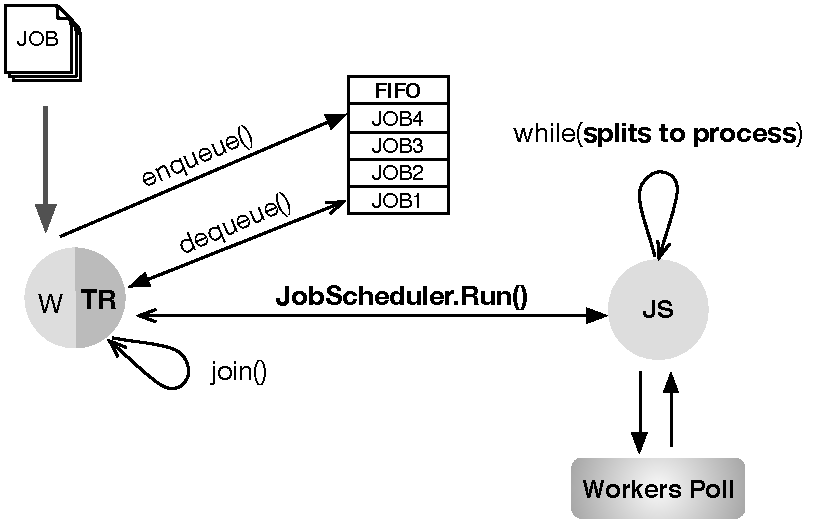
\includegraphics[width=0.48\textwidth]{pics/taskrunner-example.pdf}
                    \caption{A set of jobs are sent to an entry worker. The worker invokes a \textit{TaskRunner}, to enqueue those jobs into a FIFO queue. Then it delegates the first job's execution to a \textit{JobScheduler}, that coordinates with a pool of workers to process the job's splits.}
                    \label{fig:mnr-taskrunner-example}
                \end{center}
            \end{figure}

            \subsubsection{Task Tracker}

           In the \ac{MNRP} every worker can process only one split at a time. Therefore, after receiving a split to process by a given \textit{TaskRunner}, the worker invokes a \textit{TaskTracker} responsible for sending alive signals to the \textit{TaskRunner} with the identifier of the worker that is currently processing a given split. This way the \textit{TaskRunner} can determine if the worker has crashed or if it is stalling the processing of the split-strangler node.

        	\subsubsection{Job Scheduler}\label{job-scheduler}

            \textit{JobScheduler} is responsible for ensuring that all the splits of a given job are processed in order, even in the presence of failures or strangler nodes. To achieve it a \textit{JobScheduler} starts by gathering a set of available workers and distributes the splits among them, in order, i.e, given priority to the splits with a lower number. When a split is delegated to a worker, the scheduler starts tracking the alive signals from that worker and puts that split in the \textit{SplitsBeingProcessed} queue.

            After the splits distribution procedure finishes, the scheduler computes for every split being processed the time difference, between the workers last alive signal and the current time. For a difference superior to 60 seconds, the worker is assumed to be in a \textit{``not responding''} state, if otherwise the worker is assumed to be processing normally.

            The split processing operation runs asynchronously, i.e, the scheduler delegates the processing of the split to a worker and waits on an asynchronous task, for its response. After completion, the \textit{async} task removes the split from the \textit{SplitsBeingProcessed} queue and marks the worker status as \textit{``available"} for processing more splits.
            
            For crashed workers or workers that are simply taking too long to send alive signals, either because they have just crashed or simply because their network segment is functioning with high latencies, the scheduler retracts the split delegation from the failing worker. After that, the split is automatically assigned to a new worker if possible, otherwise it gets postponed in a waiting queue.
            
        \subsection{Replication}
        
            In the MapReduce base implementation, the \textit{Master JobTracker}—TaskRunner in our case—is a single point of failure, which means that if it fails the job processing fails and the client must re-execute the entire job again. In our solution we try to address this issue by providing replication functionality to our \textit{TaskRunners}. 
            
            When a \textit{TaskRunner} is created, a service called \textit{CoordinationManager} is also instantiated. It is responsible for the selection of a precomputed number of workers, that will be used as replicas of the current \textit{TaskRunner}. On those workers side, a worker thread—separated from the worker's main thread—is responsible for hosting the \textit{Slave Replica} execution logic, as we will see on \ref{slave-replica}.
         
        	\subsubsection{Coordination Manager}\label{coord-man}
            
            In our implementation, we followed a Master-Slave replication model, similar to the one proposed by Francesco Salbaroli~\cite{FrancescoSalbaroli2008}. In this approach, the \textit{CoordinationManager} is responsible for coordinating state updates of the \textit{TaskRunner} with a set of slave replicas. Each replica is able to save the latest state update of their \textit{TaskRunner}. On the other hand, those replicas periodically, send alive signals to the \textit{TaskRunner} in order to let both parties know about each other failures. This way, when a replica crashes, the \textit{CoordinationManager} can attempt to recover it, by electing a new worker to receive state updates of the \textit{TaskRunner}. And likewise, the replica can try to recover a crashed \textit{TaskRunner} if it is unable to communicate with it. To achieve this, the \textit{CoordinationManager} performs a set o steps, detailed bellow:
            
            \begin{itemize}
                
                \item[] {\bfseries Initialization:} During the initialization step the \textit{CoordinationManager} picks a set of replicas from the workers assigned to its \textit{TaskRunner}—workers assignment to a given \textit{JobTracker} will be better explained on Section~\ref{cluster-man}. After electing the workers that will be receiving state updates, known as Slave Replicas, the \textit{CoordinationManager} initializes the Slave Replica component on each worker and assigns them a priority number. These numbers define an hierarchy among those replicas, in an ascending order. 
                
                During a failure those numbers, are used to identify whose replica should attempt to recover the crashed \textit{TaskRunner} first. Along with a priority number, each replica is also given a list of their sibling replicas, used during the recovery of a \textit{TaskRunner} to enable the coordination of the process among them.
                
                \item[] {\bfseries Pick Replicas:} The replica picking process involves selecting a determined number of replicas not known \textit{a priori}. The problem faced in this selection is the following: if the amount of workers assigned to a given \textit{TaskRunner} is large—bigger than 5K, —the number of replicas is expected to be proportional to that number, but not directly, i.e, we don't want to depend on a relative measure like a percentage. If we do, for a 5K workers we would have 2.5K replicas which is absurd. Instead we used a function that enabled us to acquire a more balanced number of replicas, independently of the amount of workers involved, and which provides an ideal number of replicas when we have just one worker—the \textit{TaskRunner}— case in which we expect the number of replicas to be zero, since in that case we don't have resources to provide replication. Although, it is a very rare scenario, the properties of your formula holds and contemplates this without any added complexity. 
                
                Therefore, to find the optimum number of replicas we use the formula bellow:
                 \begingroup
                 \small  
                 \begin{equation*}
                 \begin{aligned}
                    min( & workersCount, \\ & round( ceiling(\log{workersCount})) * r\_factor))
                 \end{aligned}
                 \end{equation*}
                 \endgroup
            
                The table bellow illustrates some examples of the number of replicas required for a \textit{TaskRunner} using our equation:
            
                \begin{table}[!h]
                    \centering
                    \begin{tabular}{c c c}
                        \toprule \# workers & \# replicas & \textit{r\_~factor} \\
                        \midrule\vspace{-8pt} \\
                        1 & 0 & 1.0\\ 
                        \textless 100 & 2 & 1.0 \\ 
                        \textless 1000 & 3 & 1.0 \\ 
                        \textless 10.000 & 4 & 1.0 \\ 
                        \textless 100.000 & 5 & 1.0 \\ 
                        \bottomrule 
                    \end{tabular} 
                \end{table}
                
                \item[] {\bfseries State Updates:} In the state update procedure the \textit{CoordinatorManager} performs 3 actions \textit{(i)} it sends a list containing the current active replicas to all other replicas, so that in case of a replica failure, all replicas are informed, \textit{(ii)} the current state of the \textit{TaskRunner} is sent to all active replicas, and \textit{(iii)} the \textit{CoordinatorManager} checks whether there are replicas that stopped communicating with it. On \textit{(iii)}, when a replica failure is detected, the \textit{CoordinatorManager} fires a new thread to handle the replica recovery on a separate context, to avoid blocking the current thread, responsible for communicating state updates to other replicas.
                
                \item[] {\bfseries Alive Signals Listening:} Replicas communicate periodically with the \textit{TaskRunner} reporting they are up and running normally. This enables the \textit{TaskRunner} to keep track of crashed replicas and vice-versa.
                
                \item[] {\bfseries Crashed Replica Recoveries:} When a replica stops communicating with the \textit{TaskRunner} for more than 15 seconds, the \textit{CoordinatorManager} triggers the replica recovery procedure. That consists of selecting a new replica from the current available workers that are not already serving as replicas. The new replica receives a priority number equal to the last replica's priority number plus one. Which puts it in the end of the replication chain.
                
            \end{itemize}
            
            It's worth noting that, because recovered replicas are always added to the end of the replication chain and the list of active replicas is periodically updated to all replicas, if a master replica fails, the next replica in the chain is automatically promoted to master replica. Therefore, enabling fault-tolerance even over the fault-tolerance mechanism.
        	
        	\subsubsection{Slave Replica}\label{slave-replica}
            
            A slave replica main functions consists of receiving state updates from its \textit{TaskRunner} and sending heartbeats to it every 5 seconds. When a slave replica fails to communicate with its \textit{TaskRunner} it starts incrementing a counter of failed attempts. When that counter reaches a certain threshold the \textit{Master JobTracker} procedure is initiated.
            
            During the recover procedure the master replica, waits for all replicas to report the last received state of their \textit{TaskRunner}. And when it receives all states, the most up-to-date gets selected by the master replica. With the most recent state, the master replica promotes itself to master with the latest state received by all replicas.
            
            After taking the crashed \textit{TaskRunner's} place, the replicas detect that the \textit{TaskRunner} is online again, and start sending heartbeats to it, like if nothing had happened. Any current job splits sent during the failure are assumed to have been lost due to their workers failure, and are reassigned to new workers. Therefore enabling the job processing to proceed without noticing any failure.
    	
    	\subsection{Cluster Resource Management} \label{cluster-man}
            Our solution for resource management was built based on a simpler version of Facebook Corona~\cite{Facebook2012}.
            We developed it by implementing a Fair Share Scheduler, detailed in Section~\ref{fairshare}. The basic idea is,
            if there are no Job Tracker executing on the \ac{MNRP}, the first Job Tracker gets a share containing all the available workers on
            the server node where it is located. Subsequent Job Trackers that arrive at the system, ask for an equal share to process their jobs,
            i.e, if there are four Job Trackers, one forth of the workers should be given to each Job Tracker. When this isn't possible, due to lack
            of available workers at the Job Tracker's server node, the Job Tracker borrows workers from other server nodes, to process its job's.
            Finally, if there are not enough workers available in all server nodes to complete the share required by a Job Tracker, that Job Tracker is put
            on a waiting queue, until there are enough resources for it to operate.
        
            \subsubsection{Fair Share Scheduler}\label{fairshare}
            The Fair-Share algorithm provides a very balanced solution, both on efficiency and time taken to develop it. In our algorithm implementation,
            for resource attribution it was taken into account the known PuppetMaster and Task Runners. The algorithm is simple, and works as follows: on resources
            request, the number of available workers is divided by the number of know PuppetMaster's plus the numbers of TaskRunners. This way requests issued from one
            cluster to another, enables the requester to be given the same amount of resources as a worker, regarding the Fair-Share algorithm. This way the distributed
            resources request is answered with a larger amount of resources, that it would be, if were taken into account the workers inside de issuing cluster.

    	\subsection{Puppet Master}
        
	      Puppet Master is a component developed for testing \ac{MNRP}. To fully understand the potential of this system, we needed a tool, first to monitoring all the system, second to induce some delays and failures to see how the system behaves. The Puppet Master allows to create workers and get the overall status of the system. Additionally, allows to induce some delay on the whole system or only in some workers and even to simulate some failures freezing workers or its communication, i.e., the Job Tracker component.
          
            \subsubsection{Management Interface}
            
            The interface of Puppet Master it is provided of a script parsing system, which allows the user to introduce some commands through script that can be processed in batch or step-by-step. The user can load and save his scripts. The interface also has an Help menu that helps to build commands providing their syntax and for the monitoring it shows up a list of the components of the system, their status and a log window.
            
            \subsubsection{Create Worker}
            
            The create worker command instantiates a Worker with a given \emph{ID} and registers it on a given \emph{Service URI} associated to the given \emph{Puppet Master URL}. The parameter \emph{Entry URL}, specifies either if this new worker creation should be notified to the other workers, by calling the worker listening in this URI, or not, if it is left in blank.
            
            \subsubsection{Status}

            The status command \emph{STATUS} prints the \emph{ID} and \emph{Status} of all workers. This \emph{Status} can be  \emph{Busy} if the worker is processing a job, \emph{Available} if is ready to receive a job, \emph{Frozen} if a Freeze Worker command has been used (see section \ref{freeze}), or \emph{Offline}. 

            \subsubsection{Wait and Slow Worker}
            
            The Wait command allows to induce some delay to the whole system of some given seconds and it's used to give some time between two commands, for example. Note that this command is only a \emph{Thread.Sleep} to the main thread of Puppet Master. As well, the Slow Worker command induces a delay of some seconds to the given worker using the \emph{Thread.Sleep} to the main thread of that worker. This is used to simulated some slow machines that may delay the whole job processing.

            \subsubsection{Freeze/Unfreeze Worker} \label{freeze}
            
            The freeze command is used to simulate some machine that fails, helping us testing the system in a suppose real life scenario. It disables all the worker components and pauses the processing of requests. It was implemented attributing a \emph{ManualResetEvent} to every request that is received by the worker, which are set to \emph{WaitOne} when a freeze command arrives.

          \subsubsection{Freeze/Unfreeze Communication}
          
          To freeze the communication is to simulate the failure of the JobTracker component, since it is the responsible for it. When a freeze communication command is received, it is used a \emph{RemotingServices.Disconect} to avoid the component to receive any messages, as if it has failed. To recovery this component it's used a \emph{RemotingServices.Marshal} to reactivate the worker's communication.

            \subsubsection{Submit}
            
            The Submit command enables to simulate the interaction with the client. When a submit command is performed it simulates the request of a client to apply a Map function to a set of data. The client requests to a specific worker, given by the \emph{Entry Url}, to process the data contained in the \emph{File}, dividing it into \emph{S} splits which should be distributed along some workers. The map class is given by the parameter \emph{Map} which implements the \emph{IMapper} interface whose class library location is given by the \emph{Dll}. In the end, the output files should be in the give \emph{Output} folder. When a Submit command is performed, the system runs an \emph{UserApplicationSample} which instantiates a \emph{ClientService} that has two different services are available: the {\it (i)} \emph{ClientSplitProviderService} is the service that will provide the splits to the workers; the {\it (ii)} \emph{ClientOutputReceiverService} is the service that will receive the results of the map function in the end of the job processing.
            After that, the client does the \emph{SplitAndSave} of the file to process and saves it to a list that will be also send to the Master worker.
            There is a third service in the client side, {\it (iii)} \emph{OutputReadyListener} that will be waiting until the job processing is completed.
            On the Master Worker side, it is done the \emph{SplitsDelivery} through some workers and each of them asks for the data, executes the task and gives its result to the client.
            Back to the client side, the \emph{OutputReadyListener} that was waiting is \emph{Set} when all the splits' result arrive and those results are written to the \emph{Output} folder. 

	\section{Evaluation}

    All the experiments presented here have been performed in accordance to requirements presented in the Architecture section in order to show the level of their fulfillment. Our evaluation addresses the following aspects of the solution:
    
    \begin{itemize}
        \vspace{-3pt}
        \item Robustness of the fault tolerant solution and the Job-Tracker restart time
        \vspace{-6pt}
        \item State saving and message exchange overhead
        \vspace{-6pt}
        \item Scalability of the solution
                \vspace{-3pt}
    \end{itemize}

    Within our limited time frame, we had time to setup two tests scenarios \textit{(i)} the first tests the execution the job ``pl10.txt'' with a distributed load between two machines on the same network, and \textit{(ii)} we tests the same scenario in presence of a failure of the job tracker. The results acquired are presented on tables 1 and 2.

    \begin{table}
        \centering
        \label{eval1}
                                                \vspace{-10pt}
        \caption{Failure-free Test Scenario w/ 10 Workers}
    \begin{tabular}{l | c}
        \toprule
        Metrics & Statistics\\
        \midrule
        Mapper & Char Count \\ 
        Execution Time & 33 secs \\ 
        \# Messages & 3.742 \\ 
        Messages Total Size & 2.937.361 \\ 
        Result size in bytes & 100 bytes \\
        Result pairs count & 10 \\
        \bottomrule
    \end{tabular}
                                        \vspace{-10pt} 
    \end{table}

    \begin{table}
        \centering
        \label{eval2}
                                                \vspace{-10pt}
        \caption{Test Scenario w/ Job Tracker Failure}
        \begin{tabular}{l | c}
            \toprule
            Metrics & Statistics\\
            \midrule
            Mapper & Char Count \\ 
            Execution Time & 43 secs \\ 
            \# Messages & 9.158 \\ 
            Messages Total Size & 7.532.600 \\ 
            Result size in bytes & 100 bytes \\
            Result pairs count & 10 \\
            \bottomrule
            \end{tabular} 
                                    \vspace{-10pt}
            \end{table}
	\section{Conclusions}

    In this work we implemented and evaluated a design that solved the JobTracker fault tolerance and scalability problems in a way that did not significantly affect the overall system performance.
    
    The proposed design is based on saving the JobTracker state into a set of slave replicas. The JobTracker is started in the platform as a distributed task, and in case the node where it runs fails, the platform performs the JobTracker automatic failover on some other healthy node. Upon a restart, the JobTracker loads the stored state and continues with the normal operation. During the failover, TaskTrackers can continue executing the running jobs normally and the Clients and TaskTrackers automatically reconnect to the JobTracker upon the restart. In addition, the system is available for users to submit new jobs all the time.
    
    The evaluation showed that the solution does not make significant a impact on the system performance. The state saving overhead is negligible when running simple jobs and grows slowly when increasing the number and complexity of jobs.

	\bibliographystyle{splncs03}
	\bibliography{mapnoreduce-report-g03}
\end{document}